\section{16. März 2012}

\question{Diskutieren der unterschiedlichen Überlegungen in der Valenzbindungsnäherung (VB) und in der Molekularorbitalnäherung (MO) zur Beschreibung der Molekülbindung in einem 2-atomigen Molekül}
\label{q:41}

\textbf{VB-Näherung}
\begin{itemize}  
    \item erklärt Paarung von Elektronen durch Überlappung von Orbitalen ($\sigma$- und $\pi$-Bindungen)
    \item liefert KEINE Details über Molekülorbitale
    \item im Grundzustand können zwei Elektronen mit $\uparrow \downarrow$ Spins untergebracht werden
    \item zwei \textbf{lokalisierte} Elektronen um Kerne A und B
    \item beide Elektronen werden betrachtet, sodass für beide Wahrscheinlichkeitsamplituden $\psi_1$ und $\psi_2$ ein Produktansatz der Atomorbitale notwendig ist
    \item Besetzung des Molekülorbitals wird mit Linearkombination von $\psi_1$ und $\psi_2$ durch Pauli-Prinzip erzwungen
    \item \textbf{$e^-$ lokalisiert}
\end{itemize}
2 $e^-$ werden zugleich beschrieben:
\[\psi_1(\vb{r_1},\vb{r_2}) = c_1 \phi_A(\vb{r_1}) \cdot \phi_B(\vb{r_2})\]
\[\psi_2(\vb{r_1},\vb{r_2}) = c_2 \phi_A(\vb{r_2}) \cdot \phi_B(\vb{r_1})\]
und danach symmetrisch/antisymmetrisch kombiniert: 
\[\psi_{\text{sym}} (\vb{r_1},\vb{r_2}) = \psi_1(\vb{r_1}) + \psi_2(\vb{r_2})\]
\[\psi_{\text{asym}}(\vb{r_1},\vb{r_2}) = \psi_1(\vb{r_1}) - \psi_2(\vb{r_2})\]

\noindent
\textbf{MO-Näherung}
\begin{itemize}
    \item basiert auf bindenden und antibindenden Molekülorbitalen
    \item erklärt die Hybridisierung der Orbitale
    \item ein Elektron betrachtet, dass sich in $\phi_A$ als auch in $\phi_B$ aufhalten kann, sodass für dieses ein Molekülorbital-Ansatz notwendig ist (wobei $\phi_A$ und $\phi_B$ atomare Wellenfunktionen)
    \item für Besetzung des Molekülorbitals mit zwei Elektronen wird Produktansatz verwendet
    \item \textbf{$e^-$ delokalisiert}
\end{itemize}
$e^-$ werden einzeln beschrieben als Linearkombination der Atomorbitale (LCAO):
\[\psi_{e_1}(\vb{r}) = c_1 \cdot \phi_A(\vb{r}) +c_2 \cdot \phi_B(\vb{r})\]
2 $e^-$ werden mittels Produktansatz kombiniert:
\[\psi(\vb{r}) = \psi_{e_1}(\vb{r}) \cdot \psi_{e_2}(\vb{r}) \]

\question{Skizzieren der bindenden und antibindenden Wellenfunktionen in einem homonuklearen 2-atomigen Molekül}
\label{q:42}
\begin{figure}[H]
    \centering
   \begin{minipage}[b]{.4\linewidth} % [b] => Ausrichtung an \caption
      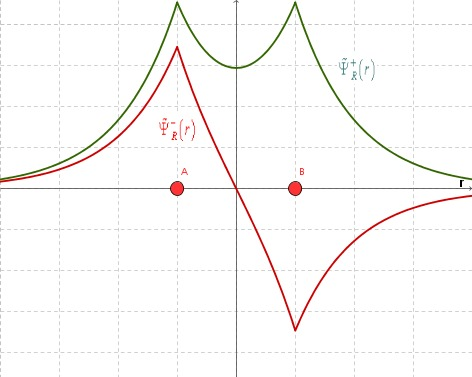
\includegraphics[width=\linewidth]{resources/16-03-2012/sym_und_antisymm_Wellenfunktion.jpeg}
      \caption{\textbf{Wellenfunktionen} symmetrische (bindend, grün) und antisymmetrische (antibindende, rot) Wellenfunktion}
   \end{minipage}
   \hspace{.1\linewidth}% Abstand zwischen Bilder
   \begin{minipage}[b]{.4\linewidth} % [b] => Ausrichtung an \caption
      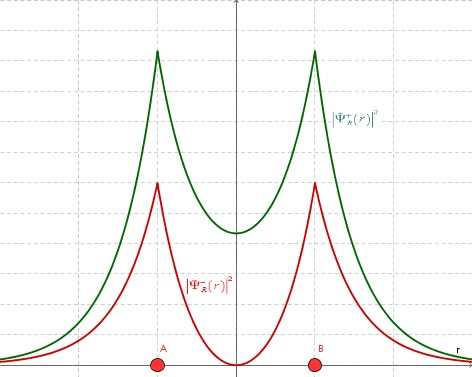
\includegraphics[width=\linewidth]{resources/16-03-2012/Wahrscheinlichkeitsdichten.jpeg}
      \caption{Wahrscheinlichkeitsdichten der symmetrischen (bindend, grün) und antisymmetrischen (antibindende, rot) Wellenfunktion}
   \end{minipage}
\end{figure}

\question{Diskutieren des Schwingungsrotationsspektrums eines 2-atomigen Moleküls}
\label{q:43}

\begin{itemize}
    \item Spektren zweiatomiger Moleküle entstehen durch Rotations- und Schwingungsübergänge
    \item im realen Molekül führen Kerne um Gleichgewichtsabstand $R_e$ Schwingungen aus, sodass sich Kernabstand $R$ während Rotation des Moleküls ändert
    \item \textbf{Rotationsspektren}
        \begin{itemize}
            \item entstehen durch Absorption des Moleküls im Infrarot-Bereich
            \item durch Energieaufnahme kommt es zu Strahlungsübergänge zwischen den Rotationszuständen
            \item in einfachster Näherung wird Molekül als \textbf{starrer Rotator} betrachtet, der sich mit konstantem Kernabstand $R=R_e$=const um Schwerpunktachse dreht. Rotationsenergie $E_{rot}$ ,als Termwert $F_{rot}$, hat bei $R=R_e$ diskrete Werte, siehe \ref{RotEnergie_starr} \ref{Termwert_RotE}. Die Abstände der Energieniveaus $\Delta E_{rot}$ nehmen linear zu, siehe \ref{Abstaende_Eniveaus_starr}.

                \begin{equation}
                E_{rot} = \frac{J(J+1)\hbar^2}{2MR_e^2}
                \label{RotEnergie_starr}
                \end{equation}

                \begin{equation}
                F_{rot} =B_eJ(J+1)=\frac{\hbar}{4\pi cMR_e^2}J(J+1) \hspace{5mm} \left[cm^{-1}\right]
                \label{Termwert_RotE}
                \end{equation}

                \begin{equation}
                \Delta E_{rot}=E_{rot}(J+1)-E_{rot}=\frac{(J+1)\hbar^2}{I}
                \label{Abstaende_Eniveaus_starr}
                \end{equation}

            \item beim \textbf{nicht-starren Rotator} (Zentrifugalkraft berücksichtigt) besteht elastische Bindung zwischen Atomen mit Federkonstante k. Der Kernabstand vergrößert sich von $R_e$ auf $R$, dabei wird das Trägheitsmoment $I=MR^2$ größer und die Rotationsenergie $F_{rot}$ kleiner, siehe \ref{RotE_nichtstarr}. Die Spektrallinien rücken mit steigender Rotationsquantenzahl J=0,1,2,... weiter auseinander. Im Vergleich zum starren Rotator liegen sie jedoch näher beisammen.
                \begin{equation}
                   F_{rot}=B_eJ(J+1)-D_eJ^2(J+1)^2+...
                   \label{RotE_nichtstarr}
                    \end{equation}
    \begin{figure}[H]
    \centering
   \begin{minipage}[b]{.3\linewidth}
      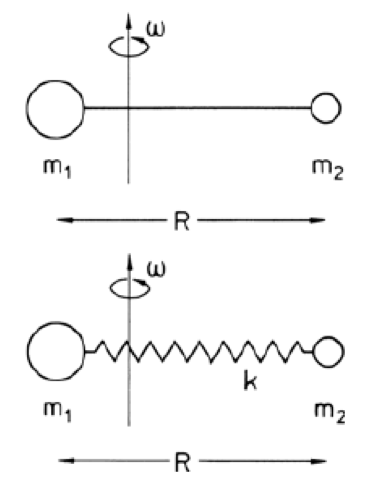
\includegraphics[width=\linewidth]{resources/16-03-2012/StarrervsnichtstarrerRotor.png}
      \caption{starrer Rotor vs nicht starrer Rotor}
   \end{minipage}
   \hspace{.1\linewidth}
   \begin{minipage}[b]{.3\linewidth} 
      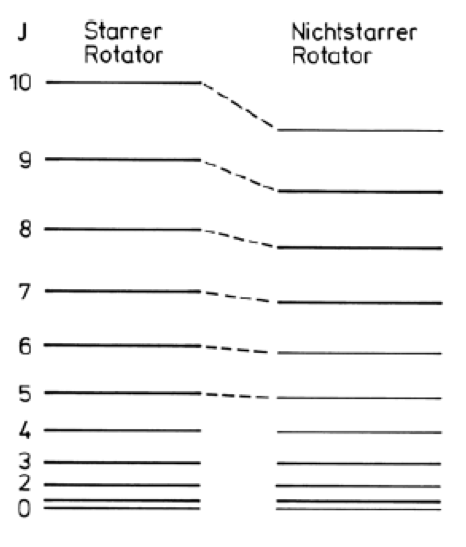
\includegraphics[width=\linewidth]{resources/16-03-2012/2starrervsnichtstarrerrotos.png}
      \caption{Übergänge starrer vs nicht starrer Rotor}
   \end{minipage}
    \end{figure}
                
        \end{itemize}

    \item \textbf{Rotationsschwingungsspektren}
        \begin{itemize}
            \item entstehen durch Absorption/Emission des Moleküls im Infrarot-Bereich, wobei Rotation und Schwingung gleichzeitig verändert werden
            \item jede Bande des Rotationsschwingungsspektrums entspricht einem Schwingungsübergang
            \item in einfachster Näherung bilden schwingende Atome des Moleküls einen \textbf{harmonischen Oszillator} mit diskreten Energie $E_{vib}$, siehe \ref{EVib_harmonisch}, und gleich großen Energieabstände $\Delta E_{vib}$, siehe \ref{EVib_Abstaende}. Potential kann durch Parabelpotential angenähert werden.

                \begin{equation}
                    E_{vib}(\nu)=(\nu+\frac{1}{2})\hbar \omega
                \label{EVib_harmonisch}
                \end{equation}

                \begin{equation}
                \Delta E_{vib}=\hbar \omega
                \label{EVib_Abstaende}
                \end{equation}

            \item bei Näherung als \textbf{anharmonischer Oszillator} rücken die Enrgieniveaus mit zunehmender Schwingungsquantenzahl $\nu$=0,1,2,... näher zusammen und konvergieren gegen Dissoziationsenergie des Moleküls. Potential kann durch Morse-Potential (\autoref{eq:morse_potential}) angenähert werden.
            \begin{equation}
                \label{eq:morse_potential}
                U(r) = U_0 \left( e^{-2(r-r_0)/a} - 2e^{-(r-r_0)/a} \right)
            \end{equation}
        \end{itemize}

\end{itemize}


\begin{figure}[H]
    \centering
   \begin{minipage}[b]{.4\linewidth}
      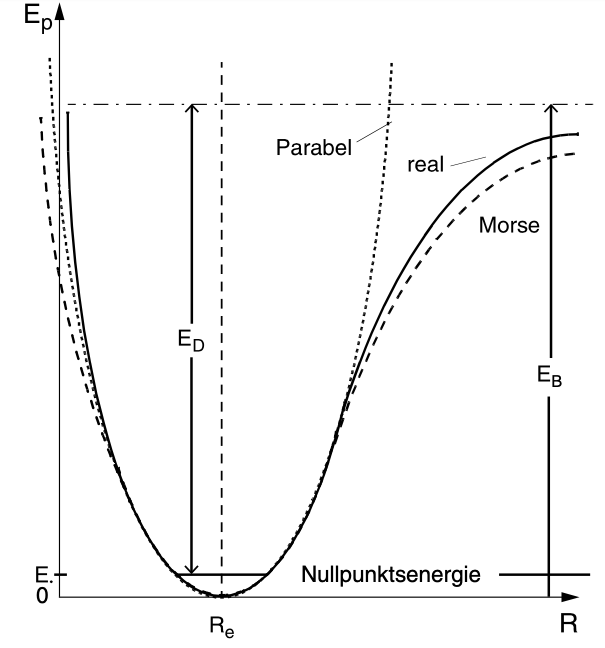
\includegraphics[width=\linewidth]{resources/16-03-2012/Vergleich_ParabelMorseReal.png}
      \caption{Vergleich zwischen Parabel-, Morse- und realen Potentials}
   \end{minipage}
   \hspace{.1\linewidth}
   \begin{minipage}[b]{.4\linewidth} 
      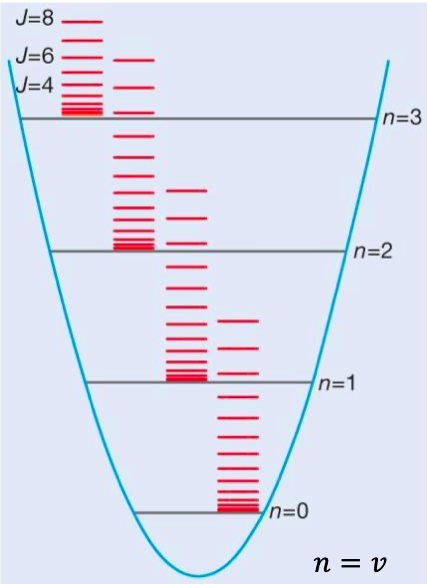
\includegraphics[width=0.8\linewidth]{resources/16-03-2012/SchwingugsRotatioinsspektrum.png}
      \caption{Darstellung der Rotations- und Schwingungsniveaus, jedem Schwingungsniveau ist Reihe von Rotationsniveaus zugeordnet}
   \end{minipage}
    \end{figure}


\question{Diskutiere die chemische Bindung im \ch{Li2}-Molekül}
\label{q:44}

Jedes Lithium-Atom liefert jeweils 3 Elektronen, insgesamt also 6 Elektronen. 
Somit sind die Molekülorbitale
\[\ch{Li2} : (1\sigma_g)^2 ~ (1\sigma_u^*)^2 ~ (2\sigma_g)^2\]
besetzt. 
Da das $(2\sigma_g)$-Orbital als höchstes besetzt ist, handelt es sich um eine stabile Bindung. 
Es gibt ein bindendes Elektronenpaar und daher handelt es sich um eine kovalente Bindung.

\textbf{Energie-Orbital-Diagram:} Am besten noch ein Energieniveau-Orbital-Diagramm zeichnen, um die Bindung zu verdeutlichen. Dann kann man argumentieren, dass die Bindung stabil ist, weil das $(2\sigma_g)$-Orbital als höchstes besetzt ist und somit die Energie des Moleküls minimiert wird.

\question{Was versteht man unter dem Franck-Condon-Prinzip? Diskutiere die Intensität von Schwingungsbänden in einem Molekülspektrum bei einem elektronischen Übergang anhand des Franck-Condon-Prinzips.}
\label{q:45}

Siehe \aqref{25}.

\question{Wodurch unterscheidet sich ein fcc Gitter von einem hcp?}
\label{q:46}

fcc -- face centered cubic, hcp -- hexagonal close-packed

\begin{enumerate}
    \item Anordnung der Atome: Im fcc-Gitter sind die Atome auf den Eckpunkten eines Würfels sowie in den Zentren der sechs Flächen platziert. Im hcp-Gitter sind die Atome hexagonal angeordnet.
    \item Einheitszelle: Im fcc-Gitter ist die Einheitszelle ein Würfel, jeder Eckpunkt enthält ein Atom. Im hcp-Gitter ist die Zelle ein hexagonales Prisma, jede Basisebene enthält ein Atom.
    \item Schichtstruktur: Im fcc-Gitter gibt es \textbf{ABCABC}-Schichten. Im hcp-Gitter sind die Schichten \textbf{ABAB}-angeordnet.
    \item Komprimierung: Im fcc-Gitter beträgt $a:c = \sqrt{2}:1$. Im hcp-Gitter beträgt $a:c = \sqrt{3}:2$.
    \item Bepackungsdichte: In beiden Gittern beträgt die maximale Bepackungsdichte 0,74.
\end{enumerate}

\question{Erläutere den Atomfaktor und den Strukturfaktor bei der Röntgenbeugung.}
\label{q:47}

Siehe \aqref{27}.

\question{Skizziere die 1. Brillouin-Zone eines ebenen Parallelogrammgitters.}
\label{q:48}

Zur Erklärung der Konstruktion siehe \aqref{28}.
\begin{figure}[H]
    \centering
    \begin{samepage}
        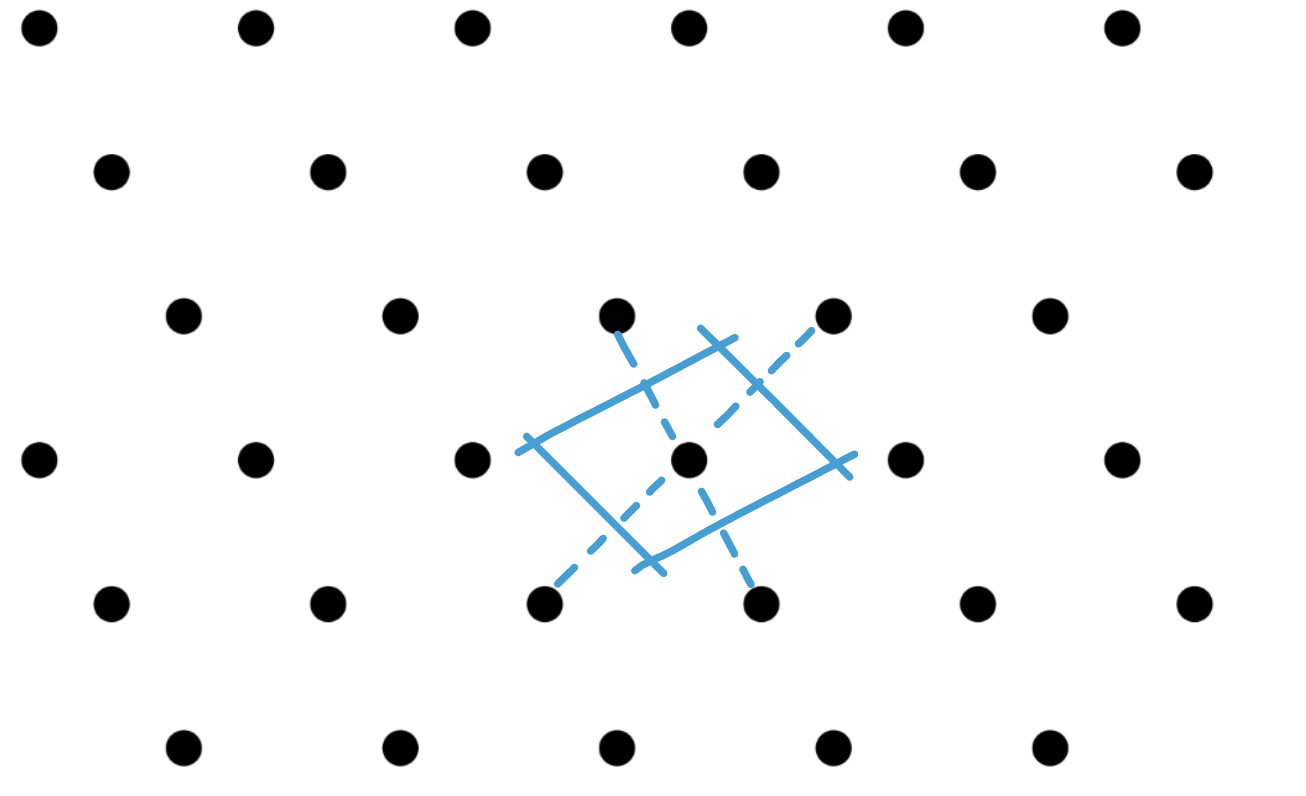
\includegraphics[width=0.4\linewidth]{resources/16-03-2012/BZ1.png}
        \caption[BZ1 Parallelogrammgitter]{1. Brillouin-Zone eines ebenen Parallelogrammgitters}
        \label{fig:BZ1_Parallelogrammgitter}
    \end{samepage}
\end{figure}

\question{Wodurch unterscheidet sich die Dispersionsrelation der Phononen eines primitiven kubischen Gitters von jener eines \ch{CsCl}-Gitters.}
\label{q:49}

\textbf{TL;DR:} Bei primitiv kubischem Gitter haben alle Atome die gleiche Masse $M_n = M$.
Es kommt daher nur zu einer Bewegungsgleichung und in folge nur zu einer Lösung für die Dispersionsrelation $\omega(\vec{k})$.
Dahingegen werden beim \ch{CsCl} Gitter zwei Bewegungsgleichungen benötigt, welche zwei Lösungen für die Dispersionsrelation besitzen mit unterschiedlichen Energien.
Die Lösung mit geringerer Energie beschreibt akustische Phononen und die Lösung mit höherer Energie optische Phononen.

\textbf{TS;WR:} Die Unterschiede können gut durch die Herleitung eines eindimensionalen Kristalls gezeigt werden:\\
\begin{minipage}[t]{0.44\textwidth}
    \centering
    \begin{figure}[H]
        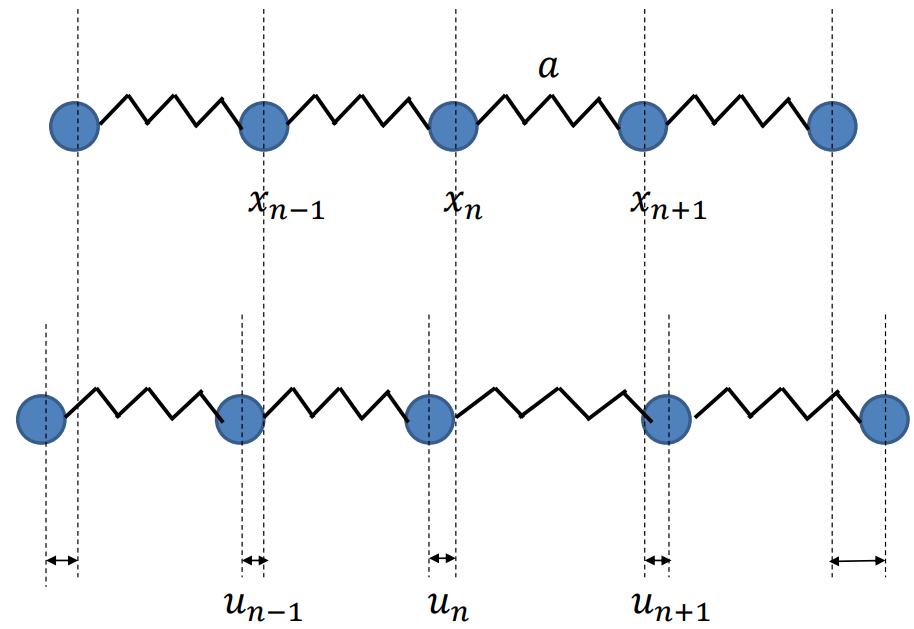
\includegraphics[width=0.7\linewidth]{resources/16-03-2012/q49_same_mass.png}
    \end{figure}
    Ausgehend von der Auslenkung $u_n$ des Atom $n$ aus der Ruhelage $x_n$ und vom Hook'schen Gesetz die Kraft $F_n$ auf Atom $n$ die aus Federverbindung mit Nachbarn resultiert:
    \begin{align*}
        u_n &= x - x_n\\
        F_n &= \sum_{p} C \left(u_{n+p} - u_n\right)
    \end{align*}
    Die Bewegungsgleichung $F_n = M \frac{d^2 u_n}{dt^2}$ ergibt sich zu:
    \begin{align*}
        M \ddot{u}_n &= C\left(u_{n+1} - u_n\right) + C\left(u_{n-1} - u_n\right)\\
        &= C\left(u_{n+1} + u_{n-1} - 2u_n\right)
    \end{align*}
    Als Lösungsansatz der DGL werden logischerweise Wellen verwendet:
    \begin{align*}
        u_n &= U_0 exp(-ikx_n)exp(-iwt)\\
            &= U_0 exp(-ikn\cdot a)exp(-iwt)
    \end{align*}
    Durch einsetzen und vereinfachen ergibt sich:
    \begin{align*}
        -M \omega^2 u_n &= C\left[exp(ika) + exp(-ika) - 2\right] u_n\\
        \rightarrow \omega(k) &= 2 \sqrt{\frac{C}{M}} \abs{sin\left(\frac{ka}{2}\right)}
    \end{align*}
    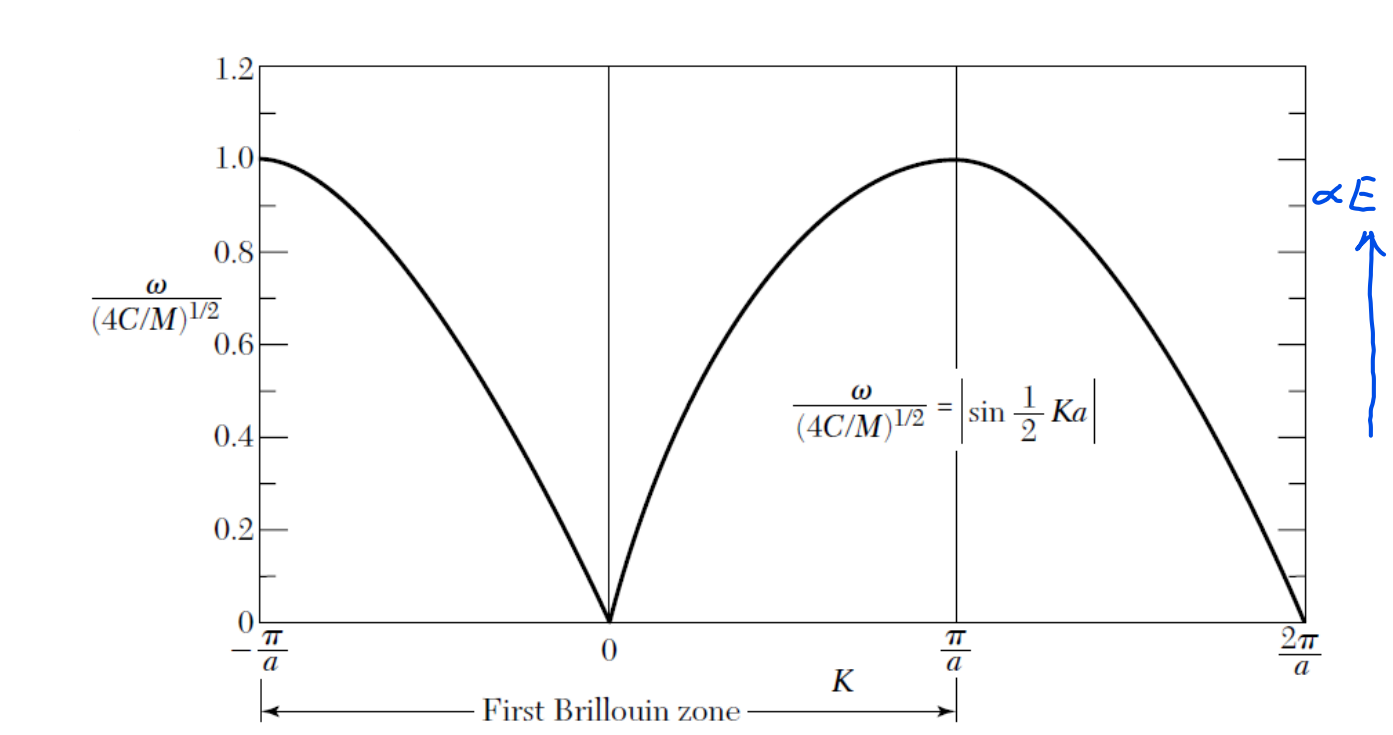
\includegraphics[width=0.9\linewidth]{resources/16-03-2012/q49_same_mass_disp.png}

\end{minipage}
\begin{minipage}[t]{0.5\textwidth}
    \centering
    \begin{figure}[H]
        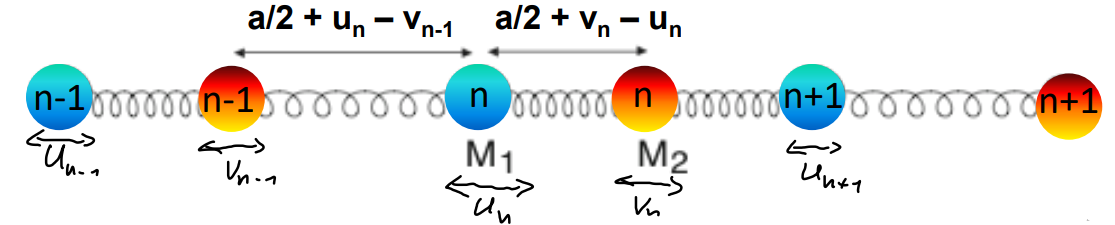
\includegraphics[width=0.9\linewidth]{resources/16-03-2012/q49_diff_mass.png}
    \end{figure}
    Achtung $a$ ist Abstand zwischen den Ruhepositionen gleich schwerer Atome (Einheitszelle).
    Bewegungsgleichungen:
    \begin{align*}
        M_1 \ddot{u}_n &= C\left(v_{n+1} + v_{n-1} - 2u_n\right)\\
        M_2 \ddot{v}_n &= C\left(u_{n+1} + u_{n-1} - 2v_n\right)
    \end{align*}
    Ansätze:
    \begin{align*}
        u_n &= U_0 exp\left(-ikn\cdot a\right)exp(-iwt)\\
        v_n &= V_0 exp\left(-ik\left[n-\frac{1}{2}\right]\cdot a\right)exp(-iwt)
    \end{align*}
    Einsetzen ergibt:
    \begin{align*}
        - M_1 \omega^2 U_0 &= 2CV_0 cos \left(\frac{ka}{2}\right) - 2CU_0\\
        - M_2 \omega^2 V_0 &= 2CU_0 cos \left(\frac{ka}{2}\right) - 2CV_0
    \end{align*}
    Durch multiplizieren (glaub ich) der beiden Gleichungen kommt man auf:
    \begin{align*}
        - M_1M_2\omega^4 - 2C \left(M_1 + M_2\right) \omega^2&\\
        + 4C^2 sin^2\left(\frac{ka}{2}\right)& = 0
    \end{align*}
    \begin{align*}
        \omega^2 &= C \left(\frac{1}{M_1} + \frac{1}{M_2}\right) \pm \sqrt{\left(\frac{1}{M_1} + \frac{1}{M_2}\right)^2} \\
        &\overline{-\frac{4}{M_1 M_2}sin^2\left(\frac{ka}{2}\right)}
    \end{align*}
    $\pm \rightarrow$ 2 Disp.rel. (Herleitung $\omega_{\pm}$ in Folien 7. Dynamik des Kristallgitters S.12-16).
    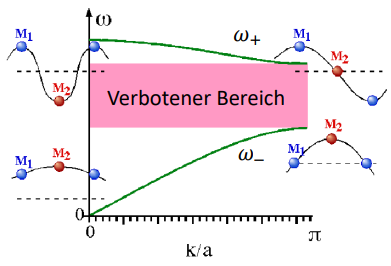
\includegraphics[width=0.7\linewidth]{resources/16-03-2012/q49_diff_mass_disp.png}
\end{minipage}

\question{Vergleiche die Einstein- und Debye-Modelle der spez. Wärme. Welche Annahme ist im Einstein Modell zu einfach?}
\label{q:50}

Siehe \aqref{40}.

\newpage